%----------------------------------------------------------------------------------------
%	ANALISI ARCHITETTURALE
%----------------------------------------------------------------------------------------

\section*{Analisi architetturale}
\addcontentsline{toc}{section}{\protect\numberline{}Analisi architetturale}%
\label{sec:analisi_architetturale}

In questo capitolo verranno presentate le decisioni architetturali inerenti la struttura e l'organizzazione del software di simulazione. L'analisi comincia con una visione generale della gerarchia di eventi, per poi suddividersi nelle scelte che riguardano la parte di concorrenza e le scelte che riguardano la parte di distribuzione.

\subsection*{Gli eventi}
\addcontentsline{toc}{subsection}{\protect\numberline{}Gli eventi}%
\label{sec:analisi_eventi}

Gli eventi sono l'elemento costituente di una partita. Essi possono essere generati dalle diverse entita' e possono essere raggruppati in diverse categorie. Inoltre, alcuni di questi eventi sono interessano la sola parte concorrente, mentre altri eventi possono viaggiare dalla parte concorrente a quella distribuita e viceversa.

\begin{figure}
	\centering
	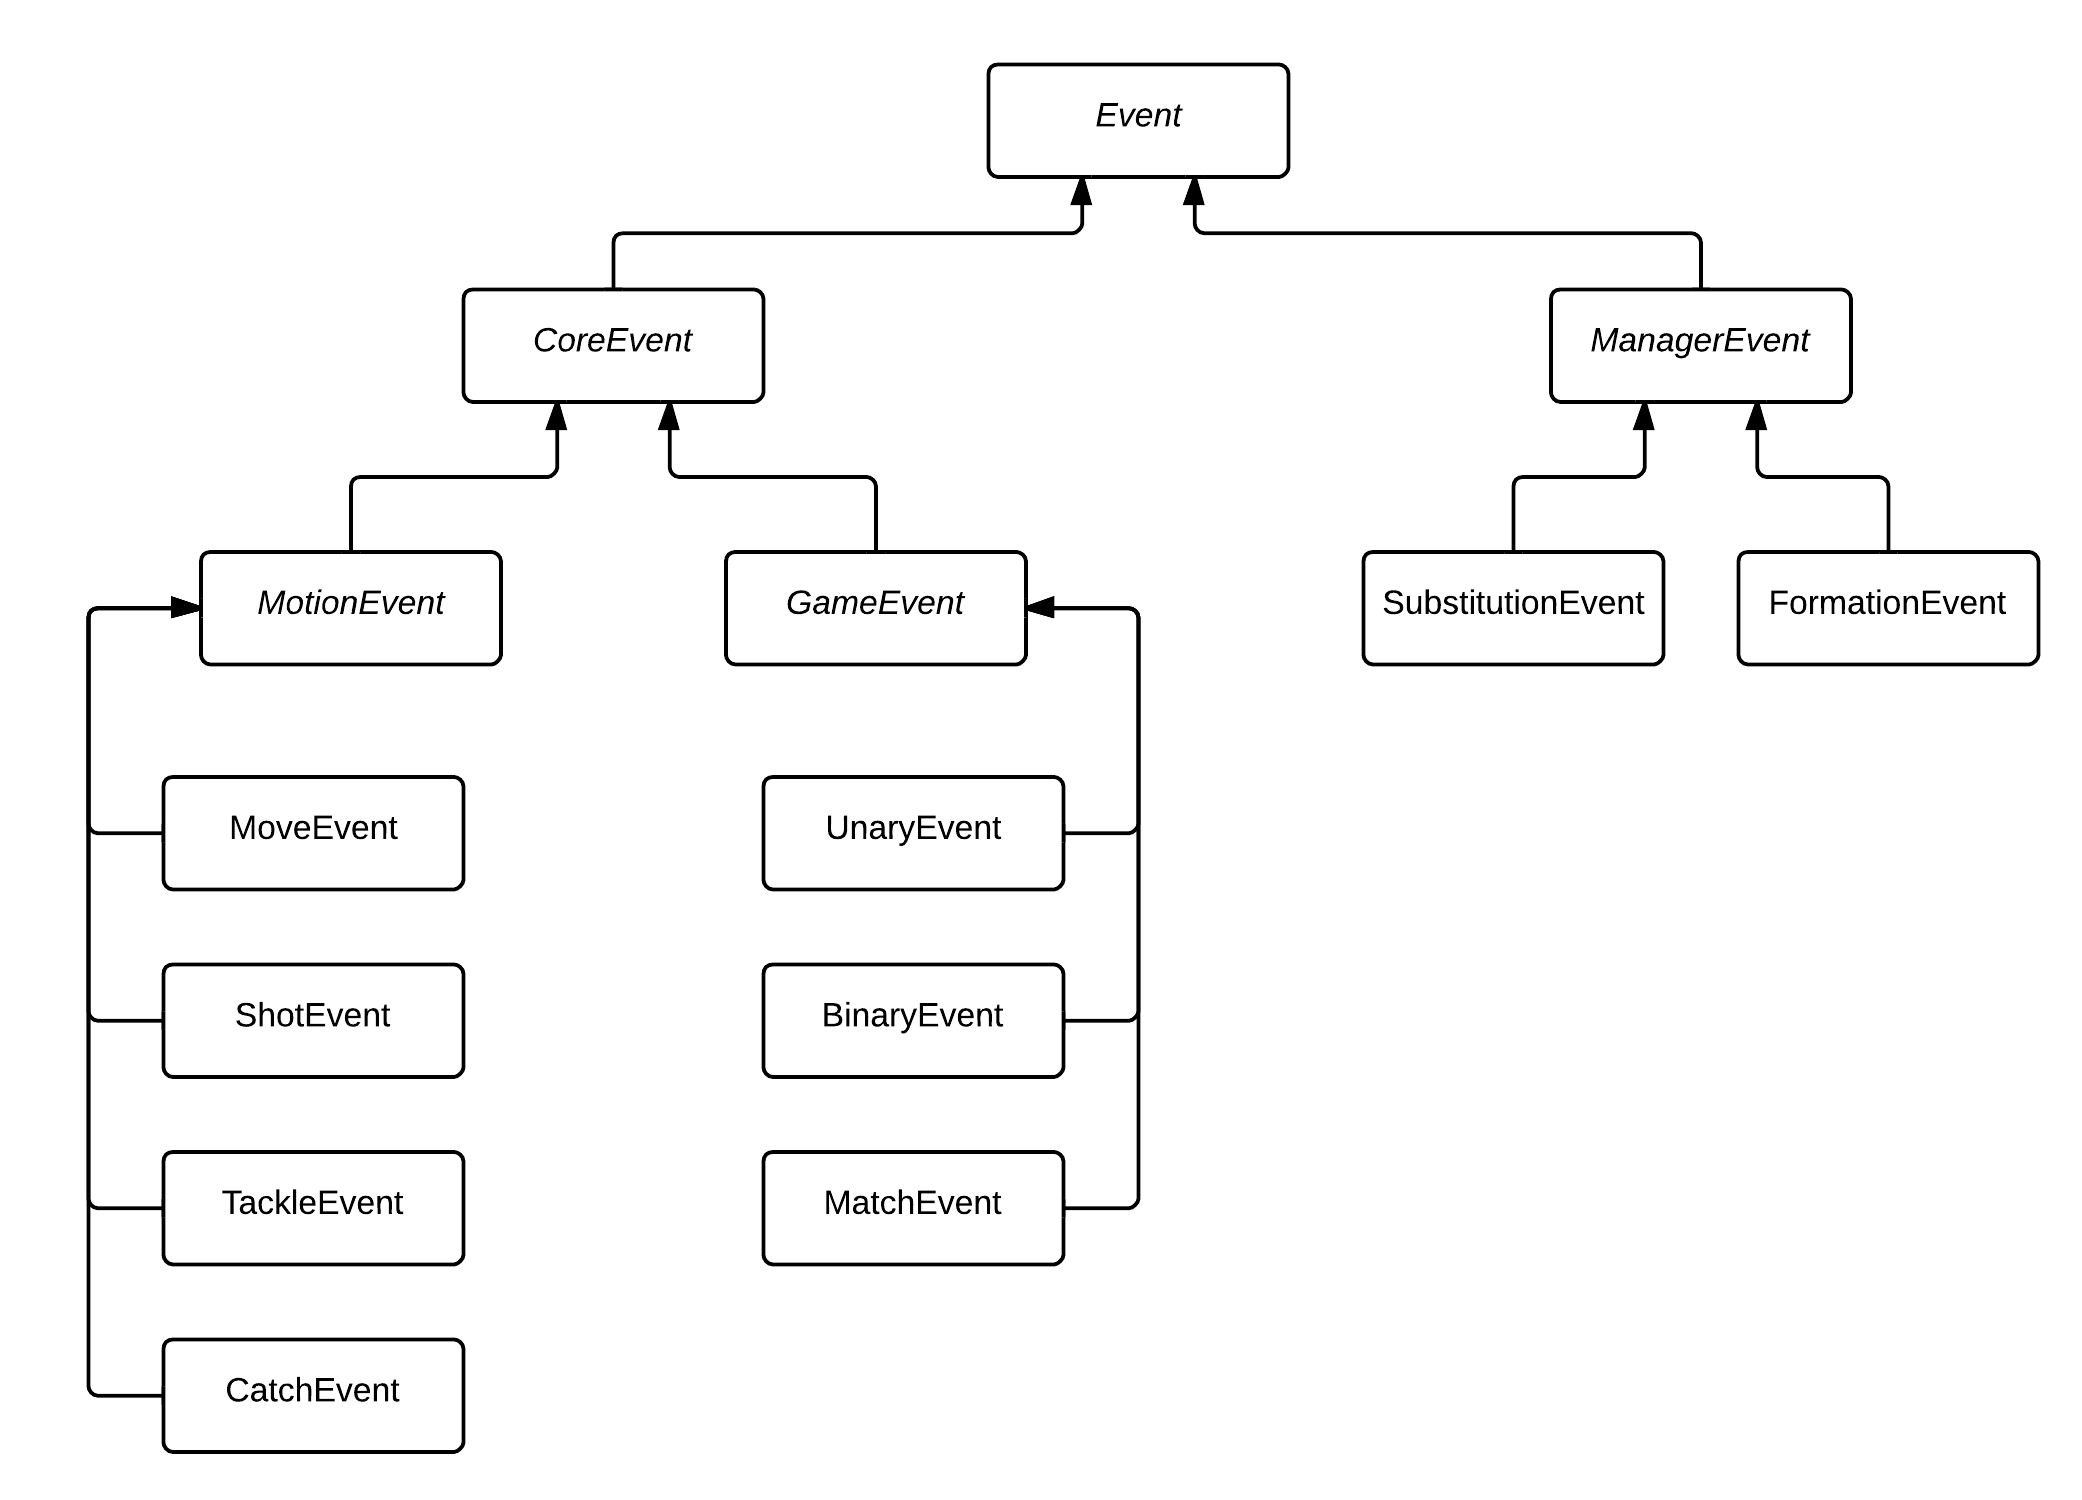
\includegraphics[scale=.5]{images/event_hierarchy.png}
	\caption{La gerarchia degli eventi che costituiscono una partita.}
	\label{fig:event_hierarchy}
\end{figure}

La struttura globale degli eventi e' schematizzata in Figura~\ref{fig:event_hierarchy}. Data la sua complessita' ed estensione, verranno ora trattati singolarmente i diversi tipi di eventi al fine di spiegarne il loro significato e il contesto in cui vengono utilizzati.

\paragraph{Event} \textit{Event} rappresenta l'evento generico ed e' alla base della gerarchia. Da esso si diramano due macro-categorie di eventi: i \textit{CoreEvent} e i \textit{ManagerEvent}. Esso sono rispettivamente gli eventi che vengono generati nella parte concorrente (il cosiddetto ``Core'') e gli eventi che vengono generati nella parte distribuita (fondamentalmente, dagli allenatori). \textit{Event} puo' essere considerata come un'entita' astratta, che non viene concretizzata se non da uno dei suoi derivati.

\paragraph{CoreEvent} Gli eventi di tipo \textit{CoreEvent} sono un insieme di eventi che vengono generati dalla parte concorrente del sistema, ovvero il Core. La loro generazione tuttavia non vincola il loro utilizzo nella sola parte concorrente: essi vengono infatti inviati alla parte distribuita per notificare gli allenatori (e l'interfaccia grafica del campo) sullo svolgersi della partita. Vi sono due tipologie di \textit{CoreEvent}: i \textit{MotionEvent}, che rappresentano le possibili azioni dei giocatori, e i \textit{GameEvent}, che invece rappresentano tutti quelli eventi che influiscono sullo stato di gioco. Anche in questo caso, i \textit{CoreEvent} sono astratti e trovano una concretizzazione nei loro discendenti.

\paragraph{MotionEvent} Tutte le azioni che un giocatore puo' compiere sono definite dai \textit{MotionEvent}. Sono stati definiti quattro tipi di \textit{MotionEvent}, elencati di seguito.

\begin{itemize}
	\item \textit{MoveEvent} - Descrivono i movimenti di un giocatore, dal punto in cui si trova al punto in cui si vuole spostare. Questi eventi vengono altresi' usati per descrivere gli spostamenti della palla.
	\item \textit{ShotEvent} - Rappresentano il tiro/passaggio effettuato da un giocatore, e sono caratterizzati da alcune informazioni quali la posizione del giocatore e la potenza impressa alla palla.
	\item \textit{TackleEvent} - Corrisponde al tentativo di contrasto verso un altro giocatore.
	\item \textit{CatchEvent} - Questo evento descrive il gesto di prendere possesso di una palla, sia essa inerte sul campo (non in possesso) oppure come intercettazione di una palla in movimento.
\end{itemize}

Ciascuno di questi eventi viene sottoposto all'attenzione dell'arbitro, che ne valida la correttezza nel rispetto delle regole del gioco. Inoltre, come gia' anticipato, questi eventi vengono anche inviati alla parte distribuita, cosi' da poter aggiornare la visualizzazione della partita e per permettere agli allenatori di prendere decisioni tattiche.

\paragraph{GameEvent} Gli eventi che regolano lo svolgimento del gioco rientrano nella categoria di \textit{GameEvent}.

\subsection*{Concorrenza}
\addcontentsline{toc}{subsection}{\protect\numberline{}Concorrenza}%
\label{sec:analisi_concorrenza}

La concorrenza.

\subsubsection*{Stato}
\addcontentsline{toc}{subsubsection}{\protect\numberline{}Stato}%
\label{sec:analisi_concorrenza_stato}

Lo stato.

\subsubsection*{Controller ed arbitro}
\addcontentsline{toc}{subsubsection}{\protect\numberline{}Controller ed arbitro}%
\label{sec:analisi_concorrenza_controller_arbitro}

Controller ed arbitro.

\subsubsection*{Giocatori}
\addcontentsline{toc}{subsubsection}{\protect\numberline{}Giocatori}%
\label{sec:analisi_concorrenza_giocatori}

Giocatori.

\subsubsection*{Palla}
\addcontentsline{toc}{subsubsection}{\protect\numberline{}Palla}%
\label{sec:analisi_concorrenza_palla}

Palla.

\subsection*{Distribuzione}
\addcontentsline{toc}{subsection}{\protect\numberline{}Distribuzione}%
\label{sec:analisi_distribuzione}

Distribuzione.


